\documentclass{article}
\usepackage{tikz}
\begin{document}
\begin{figure}[htb]
    \centering
    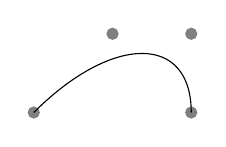
\begin{tikzpicture}
        \filldraw [gray] (0,0) circle [radius=2pt]
                         (1,1) circle [radius=2pt]
                         (2,1) circle [radius=2pt]
                         (2,0) circle [radius=2pt];
        \draw (0,0) .. controls (1,1) and (2,1) .. (2,0);
    \end{tikzpicture}
\end{figure}

\begin{figure}[htb]
    \centering
    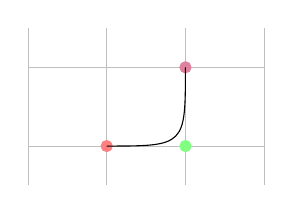
\begin{tikzpicture}
        \draw[gray!50, very thin, step=1] (2,-0.5) grid (5,1.5);
        \filldraw [red!50] (3,0) circle [radius=2pt];
        \filldraw [green!50] (4,0) circle [radius=2pt];
        \filldraw [purple!50] (4,1) circle [radius=2pt];
        \draw (3,0) .. controls (4,0) .. (4,1);
    \end{tikzpicture}
\end{figure}

\begin{figure}[htb]
    \centering
    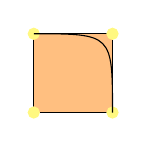
\begin{tikzpicture}
        \filldraw[draw=black, fill=orange!50] (2,0) rectangle (3,1);
        \filldraw[yellow!50] (2,0) circle [radius=2pt]
                             (3,0) circle [radius=2pt]
                             (2,1) circle [radius=2pt]
                             (3,1) circle [radius=2pt];
        \draw (2,1) .. controls (3,1) .. (3,0);                        
    \end{tikzpicture}
\end{figure}
\end{document}